\documentclass{llncs}
%
\usepackage{makeidx}  % allows for indexgeneration
\usepackage[utf8]{inputenc}
\usepackage{epstopdf}
\usepackage{float}
\usepackage{courier}
\usepackage{color}
\usepackage[usenames,dvipsnames]{xcolor}
\usepackage[export]{adjustbox}
\usepackage{graphicx}
\usepackage{hyperref}



%
\newcommand{\exedout}{%
	\rule{0.8\textwidth}{0.5\textwidth}%
}

\begin{document}
	\mainmatter              % start of the contributions
	%
	\title{WiFi Direct Multi-Group Hopping}
	%
	\author{Federico Fossemò, Gianluca Guidi}
	%
	\institute{Università di Bologna, Dipartimento di Scienze dell'Informazione
		\email{federico.fossemo@studio.unibo.it, gianluca.guidi3@studio.unibo.it}}
	\maketitle
	
	\begin{abstract}
	\end{abstract}
	%
%%%%%%%%%%%%%%%%%%%%%%%%%%%%%%%%%%%%%%%%%%%%%%%%%%%%%%%%%%%%%%%%%%%%%%%%%%%%%%%%%%%%%

%%%%%%%%%%%%%%%%%%%%%%%%%%%%%%%%%%%%%%%%%%%%%%%%%%%%%%%%%%%%%%%%%%%%%%%%%%%%%%%%%%%%%
\section{Introduzione}

\paragraph{} Questo lavoro, inserito nel contesto del corso di Sistemi Mobili, consiste nello studio di alcune potenzialità di WiFi Direct.\\
WiFi Direct consente la formazione di gruppi di comunicazione peer-to-peer. Ogni gruppo è formato da un GO (Group Owner), che agisce come access point, e più client connessi al GO. I gruppi sono indipendenti e lo standard non prevede una procedura per connettere più gruppi tra loro, per formare dei cluster più ampi.

\paragraph{} Un possibile modo per collegare più gruppi consiste nell'avere un client che si connette a più GO, rimanendo connesso a ciascuno di essi per un determinato perdiodo di tempo. Il client, saltando da un GO all'altro ed inoltrando i messaggi ricevuti, è in grado di agire da ponte tra i gruppi, permettendo lo scambio di messaggi tra dispositivi appartenenti a gruppi diversi.

\paragraph{} Lo scopo del progetto presentato è quello di fornire un proof-of-concept del metodo appena descritto, analizzare i ritardi introdotti ed eventualmente trovare un adeguato tempo di permanenza nel gruppo. L'implementazione consiste in un'applicazione Android che fa uso del framework WifiP2p fornito dalla piattaforma. Lo scenario analizzato è quello in cui sono presenti due Group Owner ed un client che si connette in alternanza ad essi.

%	\begin{enumerate}
%		\item \textit{}
%	\end{enumerate}
	
	

%%%%%%%%%%%%%%%%%%%%%%%%%%%%%%%%%%%%%%%%%%%%%%%%%%%%%%%%%%%%%%%%%%%%%%%%%%%%%%%%%%%%%
\section{Scenario del test}

\paragraph{} I dispositivi Android a disposizione per questo progetto sono 3: essi sono sufficienti per creare le condizioni minime per poter testare l'idea del salto tra gruppi: due dispositivi agiscono come Group Owner, mentre il terzo agirà come client che si connette in alternanza tra i primi due, rimanendo connesso a ciascuno di essi per un periodo di tempo prefissato.

\paragraph{} Ai due Group Owner sono stati assegnati due ruoli. Il primo, detto generator, genera periodicamente messaggi da inoltrare. Il secondo, detto replier, non fa altro che rispedire al mittente i messaggi ricevuti. Il generator prende nota dei tempi di invio e di ricezione, in modo da poter calcolare l'RTT (round trip time) presente tra sè stesso ed il replier. La stima di questo RTT è influenzata dai tempi di processamento e dal tempo di trasmissione dei messaggi. Tuttavia il tempo di processamento dovrebbe essere molto più basso rispetto ad i tempi di ritardo e trasmissione, mentre la piccola dimensione dei messaggi fa sì che la misurazione finale non venga distorta in maniera significativa.

\begin{figure}[H]
	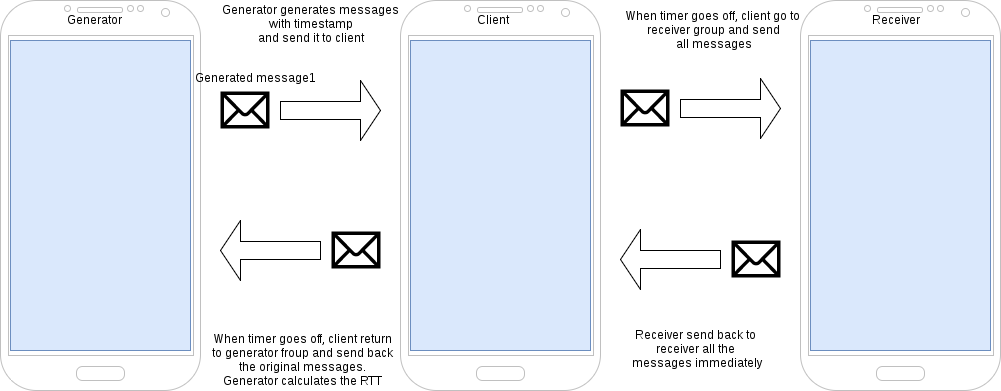
\includegraphics[scale=0.3,center]{img/archp2p.png}
	\caption{}
	\label{label}
\end{figure}
\noindent
%	\cite{relatedWork}

%	\ref{leo_arch}

%	\begin{figure}[H]
%		\includegraphics[scale=0.3,center]{img/}
%		\caption{}
%		\label{label}
%	\end{figure}
%	\noindent

%%%%%%%%%%%%%%%%%%%%%%%%%%%%%%%%%%%%%%%%%%%%%%%%%%%%%%%%%%%%%%%%%%%%%%%%%%%%%%%%%%%%%		 
\section{Architettura}

\paragraph{} In questa sezione verrà descritta a grandi linee l'implementazione dell'applicazione usata per i test. Il protocollo da noi previsto prevede diversi tipi di messaggi che possono essere inviati. Quando il client 
riesce a stabilire una nuova connessione, esso invia un messaggio di tipo REGISTER che contiene la lista dei GO raggiungibili dal client. La ricezione di questo messaggio anticipa lo scambio di messaggi di tipo DATA, il cui scopo
è solamente quello di trasmettere dati per la rilevazione delle statistiche. Quando il timer impostato dall'utente scade, il client avvia una procedura di disconnessione che consiste nell'invio di un messaggio di STOP e nella ricezione 
di un relativo STOP\_ACK. A questo punto il client è in grado di avviare la disconnessione a livello data link con la certezza di non aver perso informazioni a livello applicativo.
Le classi principali sono MainActivity, DeviceManager, Peer e MessageManager.
\begin{figure}[H]
	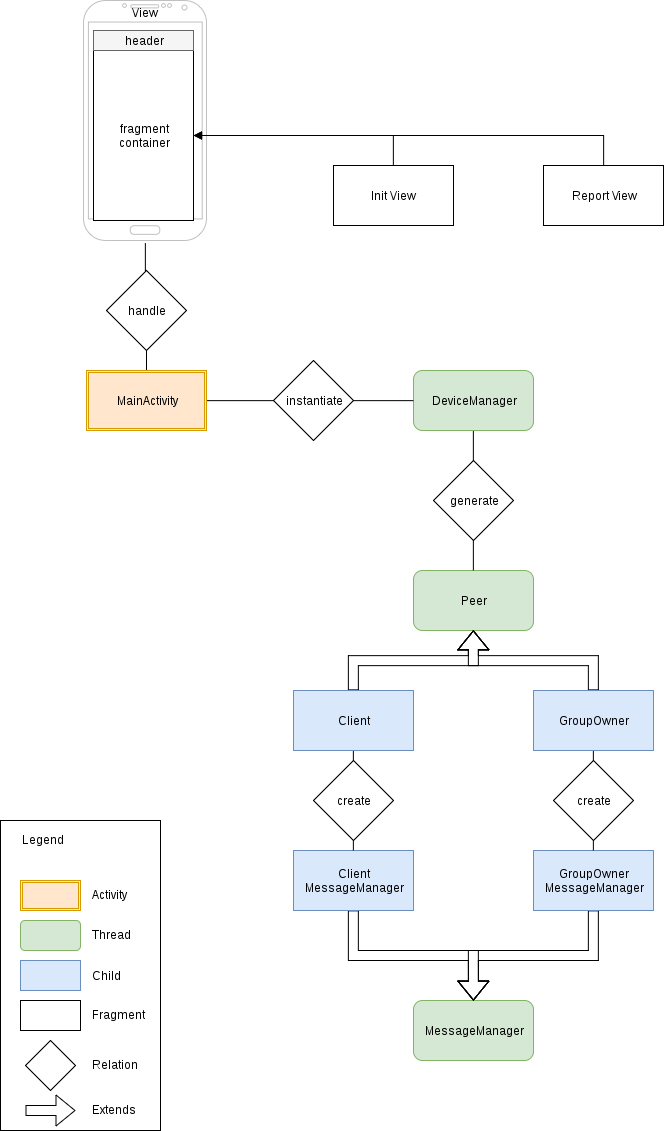
\includegraphics[scale=0.3,center]{img/class.png}
	\caption{}
	\label{class}
\end{figure}
\noindent

\paragraph{MainActivity} è un'activity che gestisce l'interfaccia grafica. L'aspetto dell'interfaccia cambia grazie all'uso dei fragment.
//TODO Fosse lascio a te la parte in cui descriviamo l'interfaccia grafica.

\paragraph{DeviceManager} è un thread che si occupa di gestire la rete a livello di WiFi Direct. Implementa varie callback che vengono chiamate quando si verificano determinati eventi.
Ad esempio \emph{onConnectionInfoAvailable()} viene chiamata quando alcune informazioni sulla connessione sono disponibili: questo significa che la connessione è stata stabilita.
\emph{DeviceManager} si occupa anche di istanziare una delle due sottoclassi di Peer (\emph{GroupOwner} e \emph{Client}) a seconda del ruolo che il dispositivo deve svolgere. Questi oggetti vengono informati sui cambiamenti della connessione, in particolare su quando essa viene stabilita.

\paragraph{Peer} è una classe astratta che rappresenta un peer, sia esso GO o client. Il suo compito è quello di rispondere al completato stabilimento di una nuova connessione (\emph{onConnect()}), 
di gestire i messaggi ricevuti (\emph{receiveMessage()}) e di gestire la procedura di disconnessione (\emph{initiateDisconnection()} e \emph{onDisconnect()}). 
\emph{Peer} genera anche un'istanza di una sottoclasse di \emph{MessageManager} (\emph{GroupOwnerMessageManager} o \emph{ClientMessageManager}).

\paragraph{MessageManager} è un thread che gestisce la ricezione e l'invio dei messaggi. L'invio dei messaggi è inoltrato ad un thread \emph{Sender} generato appositamente dal \emph{MessageManager}. Il motivo dell'esistenza di due thread, per ricezione ed invio di messaggi, risiede nella possibilità di eseguire le due operazioni contemporaneamente senza bloccarsi, in particolare per non rischiare di perdere informazioni in arrivo. Il \emph{Sender} mantiene 
una coda di messaggi da inviare. La procedura di disconnessione prevede l'invio di un messaggio (STOP per il client e STOP\_ACK per il GO); questo messaggio deve essere l'ultimo inviato, perciò è anche previsto un meccanismo che 
permette al thread di aspettare fino a quando la coda dei messaggi da inviare non sia vuota.

\paragraph{GroupOwner} una sottoclasse di \emph{Peer} che rappresenta un Group Owner. Il GO può assumere il ruolo di generator o di replier; questo ruolo può essere cambiato anche dopo la creazione. Se il ruolo è quello di generator, 
dopo aver ricevuto il messaggio REGISTER dal client, verrà avviata la generazione dei messaggi all'interno del \emph{GroupOwnerMessageManager}. La raccolta delle statistiche viene effettuata dal generator all'invio e alla ricezione dei messaggi.

\paragraph{GroupOwnerMessageManager} è una sottoclasse di \emph{MessageManager} che si occupa dell'invio e della ricezione dei messaggi da parte del GroupOwner. Questa classe viene istanziata solo una volta nel momento in cui 
il dispositivo diventa un GO: viene creato un ServerSocket, poi ad ogni connessione viene creato un socket associato al client. Se il GO è un generatore, quando viene stabilita un connessione il\emph{GourpOwnerMessageManager} lancia 
un thread \emph{MessageGenerator} che non fa altro che generare nuovi messaggi ed inviarli con una frequenza prefissata (100 ms). Quando viene effettuata la disconnessione il \emph{MessageGenerator} viene terminato.

\paragraph{Client} una sottoclasse di \emph{Peer} che rappresenta un client. Quando è stata stabilita una nuova connessione a livello di WiFi Directi il client lancia un'istanza di \emph{ClientMessageManager}, la quale dà inizio allo 
scambrio di messaggi. Viene mantenuta una coda per ogni GO, 
in cui il client memorizza i messaggi ricevuti. Le code sono indicizzate in base al MAC address della destinazione. Quando il client si connette ad un GO la cui coda non è vuota, esso invia immediatamente tutti i messaggi al GO al 
fine di svuotare la coda. Quando il tempo allocato alla connessione scade, il client dà inizio alla procedura di disconnessione inviando un messaggio STOP. Al momento della ricezione del messaggio STOP\_ACK il client avvia 
la disconnessione a livello di WiFi Direct. Il client prende nota del tempo di riconnessione, ovvero il tempo che intercorre tra l'inizio della disconnessione da un GO all'avvenuta connessione con un altro GO. La misura ottenuta non 
tiene conto del tempo necessario a stabilire una connessione TCP.

\paragraph{ClientMessageManager} è una sottoclasse di \emph{MessageManager} il cui scopo è gestire l'invio e la ricezione dei messaggi da parte del Client. Questo thread viene rilanciato ogni volta che viene stabilita una nuova 
connessione e viene terminato al termine della connessione. Questa scelta è dettata dal fatto che il socket è associato ad una connessione, quindi è più semplice gestirlo in questo modo. È stato utilizzato un thread pool per minimizzare 
il tempo di creazione del thread. Il client dà inizio allo scambio di messaggi inviando un messaggio REGISTER contenente la lista di GO nelle vicinanze. Vengono gestiti l'invio e la ricezione dei messaggi come descritti in 
\emph{MessageManager} e \emph{Client}.

\subsection{TCP e UDP}
\paragraph{} All'interno di questo progetto sono stati considerati due protocolli di trasporto: TCP e UDP. Ci sono ragioni valide per utilizzare entrambi i protocolli.
\paragraph{} La scelta di TCP, che fornisce uno stream affidabile di dati, può essere argomentata col fatto che è piuttosto comune per molte
tipologie di applicazioni si aspettino che venga fornito questo tipo di servizio. Ovviamente ci sono alcune eccezioni, specialmente quando i requisiti di
latenza sono particolarmente stretti. Tuttavia questo protocollo non si comporta in maniera ottimale quando utilizzato su una tecnologia trasmissiva a livello fisico di tipo wireless.
\paragraph{} Nel caso specifico del progetto, UDP è stato ritenuto più adatto a misurare la latenza, in quanto il protocollo non introduce ritardi sostanziali.
La scelta di utilizzare UDP richiede nella maggior parte dei casi lo sviluppo di un protocollo complementare di livello applicativo, per gestire perdite e/o ordine dei pacchetti.
\paragraph{} È stato deciso che invece di scegliere ed implementare solo uno dei due protocolli, sarebbe stato più interessante realizzare due implementazioni alternative che ne fanno uso, per poi confrontare i risultati. Sono quindi state realizzate due diverse implementazioni. Tuttavia è stato riscontrato un
problema nella versione con UDP. La API Android per WiFi Direct fornisce un metodo \emph{disconnect()} che consente al client di scollegarsi da un gruppo. La chiamata di questo metodo è necessaria affinché il client possa disconnettersi e riconnettersi ad un gruppo diverso. Vengono definite due callback che vengono
chiamate in base all'esito di \emph{disconnect()}: \emph{onSuccess()} e \emph{onFailure()}. Nell'implementazione con UDP, la chiamata di \emph{disconnect()}
non ha alcun effetto: non viene chiamata nessuna delle callback e lo stato della connessione non viene modificato. Questa è una delle tante testimonianze
dell'instabilità del framework fornito da Android. Dato che il debug del framework è stato considerato al di fuori della portata di questo progetto,
l'implementazione con UDP è stata infine abbandonata, e tutti i test sono stati effettuati utilizzando TCP.
		
%%%%%%%%%%%%%%%%%%%%%%%%%%%%%%%%%%%%%%%%%%%%%%%%%%%%%%%%%%%%%%%%%%%%%%%%%%%%%%%%%%%%%
\section{WiFiP2P API} 
\paragraph{}In questa sezione verranno descritte le API fornite da Android che sono state utilizzate per permettere l'uso della tecnologia WiFi Direct. Come descritto nella documentazione ufficiale \cite{android}, queste API consistono in tre parti principali:

\begin{itemize}
	\item Il WifiP2pManager che contiene i metodi per la discovery, la richiesta di connessione e la connessione ai peer;
	\item I Listener che consentono di essere notificati sulla riuscita o meno di una chiamata di un metodo del WifiP2pManager. Questi listener vengono passati come parametri alle chiamate dei metodi.
	\item Gli Intent che permetto di essere notificati sull'avvenimento di uno specifico evento a livello WiFi P2P, come la perdita di connessione o la scoperta di un nuovo peer disponibile.
\end{itemize}
Vediamo ora nello specifico ognuno di questi tre componenti:

\paragraph{WifiP2pManager}
È la classe che fornisce i metodi che consentono di interagine con l'hardware WiFi. I metodi disponibili sono:
\begin{itemize}
	\item{initialize()} Registra l'applicazione con il framework WiFi P2P. Deve essere chiamata prima di ogni altro metodo.
	\item{connect()} Utilizzato per connettersi ad un device con le configurazioni passate.
	\item{cancelConnect()} Cancella tutte le negoziazioni in corso per la formazione di un gruppo.
	\item{requestConnectInfo()} Richiede le informazioni di connessione del dipsositivo.
	\item{createGroup()} Crea un gruppo P2P con il dispositivo corrente nel ruolo di Group Owner.
	\item{removeGroup()} Rimuove il gruppo P2P corrente.
	\item{requestGroupInfo()} Richiede le informazione del gruppo nel quale il dispositivo è connesso.
	\item{discoverPeers()} Inzia la fase di scoperta dei peer vicini disponibili per stabilire una connessione. La discovery rimane attiva finchè non viene formato un gruppo o viene iniziata la fase di connessione.
	\item{requestPeers()} Restituisce la lista dei peer facenti parte del gruppo corrente.
\end{itemize}

\paragraph{Listener}
I listner sono interfacce che vengono passate ai metodi del WifiP2pManager per essere informati sullo stato della chiamata. I diversi metodi del WifiP2pManager accettano diversi tipi di listener:
\begin{itemize}
	\item{ActionListener} Vengono utilizzati dai metodi \textit{connect(), cancelConnect(), createGroup(), removeGroup(), discoverPeers()} e prevedono due metodi: onSuccess() che notifica l'esecuzione corretta del metodo e la onFailure() che informa la non riuscita dell'operazione fornendo anche un intero che identifica la ragione.
	\item{ChannelListener} Utilizzato dalla \textit{initialize()} e notifica sulla perdita di un canale attraverso la onChannelDisconnected().
	\item{ConnectionInfoListener} Attraverso la onConnectionInfoAvailable() notifica la disponibilità delle informazioni del gruppo richieste dalla \textit{requestConnectInfo()}.
	\item{GroupInfoListener} Attraverso la onGroupInfoAvailable() notifica che le informazioni del gruppo P2P richieste dalla \textit{requestGroupInfo()} sono disponibili.
	\item{PeerListListener} Fornisce l'informazione, attraverso la onPeersAvailable(), che la lista dei peer richiesta dalla \textit{requestPeers()} è disponibile.
\end{itemize}

\paragraph{Intent}
Gli Intent sono messaggi asincroni di cui viene fatto broadcast quando un determinato evento WiFi P2P avviene, come ad esempio la scoperta di un  nuovo peer o il cambio di stato del dispositivo. Per abilitare la ricezione di questi tip di messaggi bisogna registrare l'applicazione creando un Broadcast receiver che gestisce i seguenti tipi di intent:
\begin{itemize}
	\item{WIFI\_P2P\_CONNECTION\_CHANGED\_ACTION} Inviato quando lo stato wiFi del dispositivo è cambiato.
	\item{WIFI\_P2P\_PEERS\_CHANGED\_ACTION} Inviato quando si chiama la  \textit{discoverPeers()} e indica che la lista dei peer disponibile ha subito una variazione.
	\item{WIFI\_P2P\_STATE\_CHANGED\_ACTION} Indica se lo stato del WifiP2P è attivo o disattivo.
	\item{WIFI\_P2P\_THIS\_DEVICE\_CHANGED\_ACTION} Inviato quando informazioni del dispositivo sono state modificate come ad esempio il nome del dispositivo.
\end{itemize}
\paragraph{} L'utilizzo e la comprensione di queste API è stato necessario per lo svolgimento dell'esperimento. Tuttavia, la documentazione fornita non è ben dettagliata ed in molte occasioni è stato necessario scoprire in maniera empirica come funzionassero. L'ordine giusto in cui i metodi devono essere chiamati è stato trovato solamente dopo numerosi tentativi.
È stato inoltre constatato che il framework è piuttosto instabile: a volte le operazioni non vengono completate correttamente senza che venga  fornita alcuna spiegazione. In alcuni casi il comportamento del framework è addirittura in contrasto con la documentazione ufficiale. Solo a titolo di esempio si ricorda il caso già citato della \emph{disconnect()} per disconnettersi dal gruppo: in determinate condizioni non viene chiamata alcuna callback per indicare il successo o il fallimento dell'operazione, che no nviene mai portata a termine.


%%%%%%%%%%%%%%%%%%%%%%%%%%%%%%%%%%%%%%%%%%%%%%%%%%%%%%%%%%%%%%%%%%%%%%%%%%%%%%%%%%%%%			
\section{Esperimenti}
\paragraph{} In questa sezione desciveremo gli esperimenti condotti e mostreremo i risultati ottenuti da tali esperimenti. Mostreremo come il tempo di connessione ad un gruppo aggiunga un effort in termini di tempi molto elevato.
\paragraph{Scenari} Gli esperimenti effettuati miravano a trovare L'RTT di un qualsiasi messaggio al variare dello scenario. I differenti scenari differiscono tra loro nel tempo di permanenza del client in ognuno dei gruppi.I tempi di permanenza presi in considerazione sono i seguenti: \textit{1sec, 2sec, 3sec, 4sec, 5sec, 6sec, 7sec, 8sec, 9sec, 10sec, 15sec, 20sec}. Ogni esperimento nei differenti scenari è stato ripetuto 6 volte, dove per esperimento si intende il completo ciclo di connessione al generator con ricezione dei messaggi, disconnessione dal generator e connessione al receiver con invio e ricezione dei messaggi e disconnessione dal receiver e riconnessione al generator per reinviare i messaggi.
\paragraph{Risultati} I risultati delle prove effettuate sono mostrati in Fig. \ref{report}. Nella tabella vengono riportati i RoundTripTime medi (RTT Avg.), i TimeToReconnect medi (TTR Avg.) e il Delay, calcolato come la metà dell' RTT. Ciò che salta subito all'occhio è il tempo di riconnessione medio che si mantiene stabile negli intorni dei 7 secondi, variando da un 6.3345833333 ad un 8.2815 secondi. Discorso differente è se si va a valutare il valore assoluto di questo tempo in ogni esperimento. Infatti si è riscontrato che questo valore ha un comportamento altamente incostante, variando tempi di 3.356 secondi a picchi di valore pari a 16.54 (giustificati da possibili interferenze).
\begin{figure}[H]
	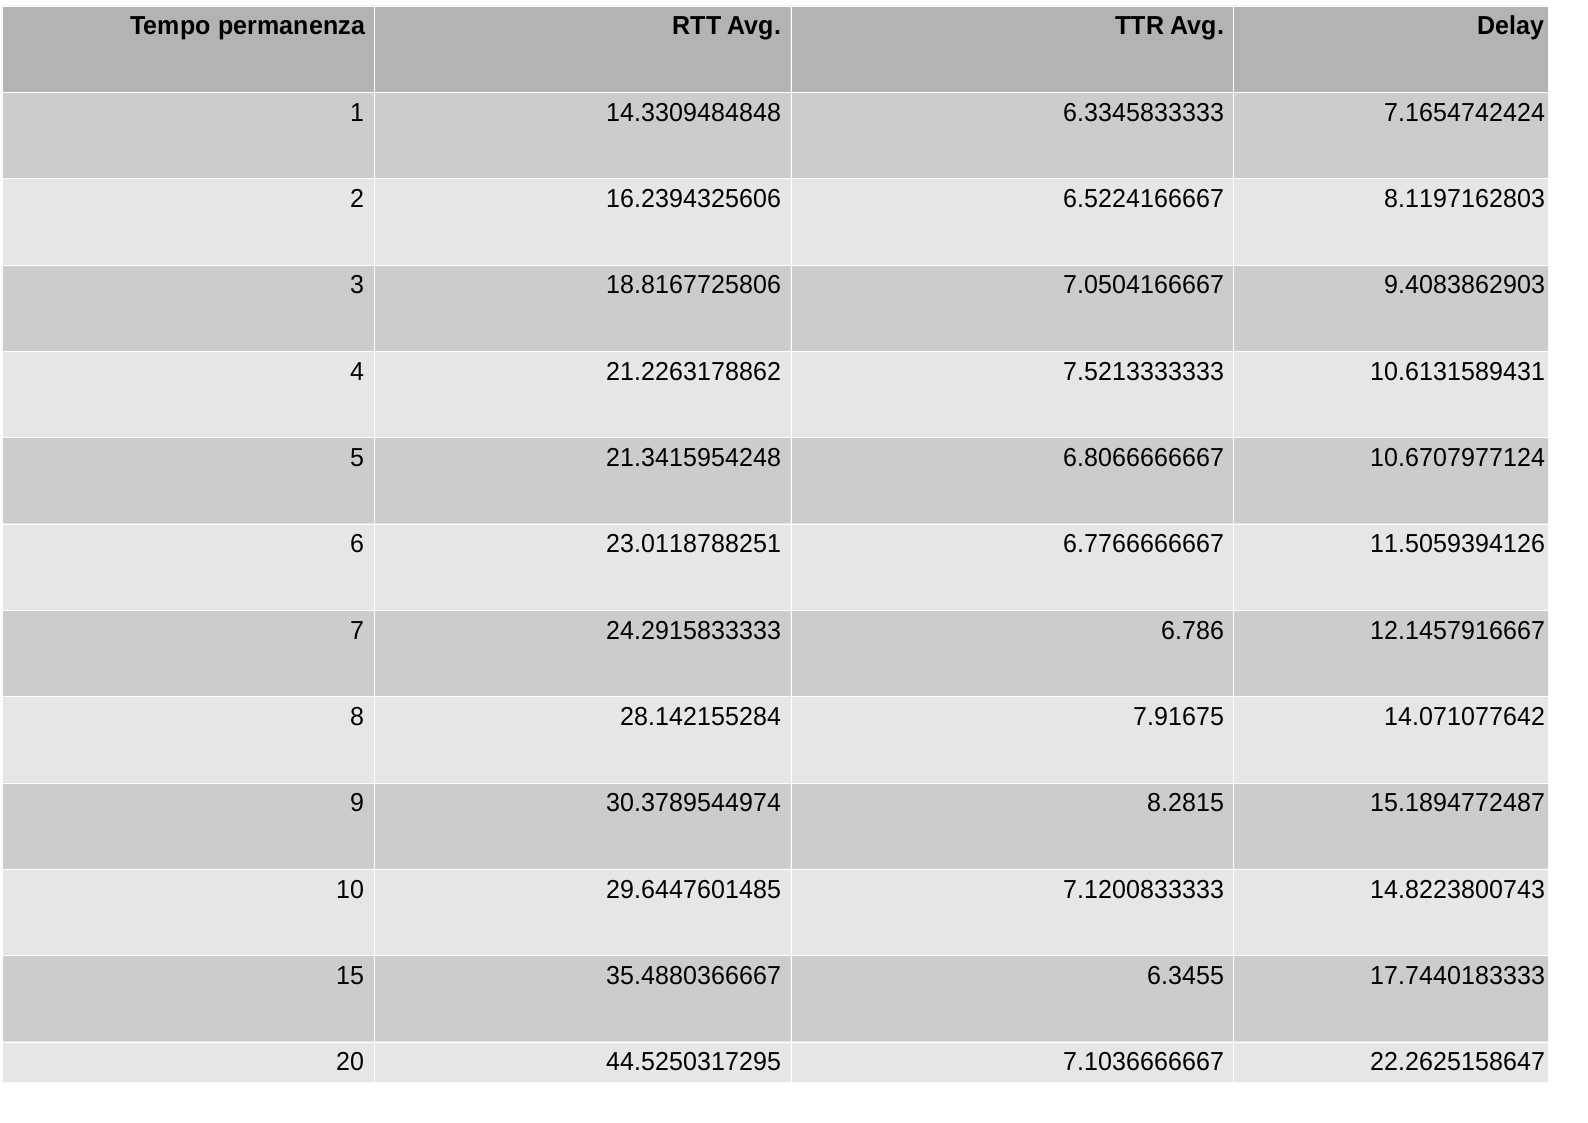
\includegraphics[scale=0.3,center]{img/report.png}
	\caption{}
	\label{report}
\end{figure}
\noindent
Dagli esperimenti effettuati si evidenziano due fatti principali come mostrato in Fig. \ref{rtt}: Il RoundTripTime (RTT) e di conseguenza il Delay aumenta con l'aumentare del tempo di permanenza del client nel gruppo P2P e che il TimeToReconnect (TTR) in media circa 7 secondi.
\begin{figure}[H]
	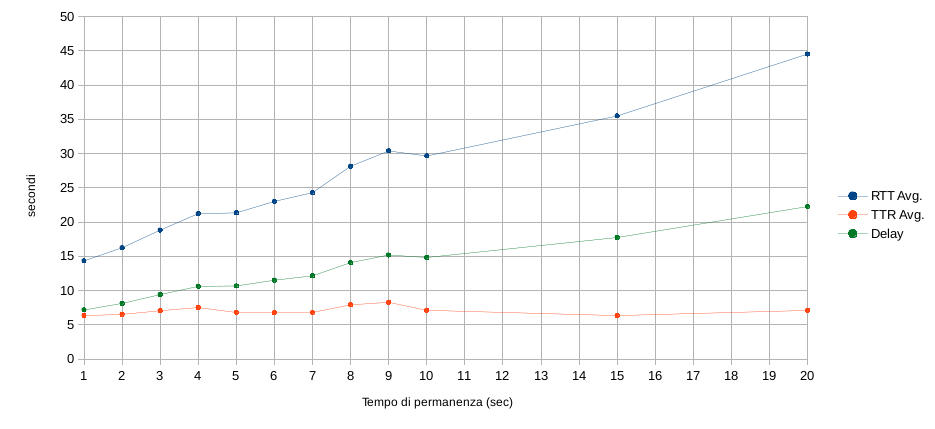
\includegraphics[scale=0.5,center]{img/rtt.png}
	\caption{}
	\label{rtt}
\end{figure}
\noindent
	
%%%%%%%%%%%%%%%%%%%%%%%%%%%%%%%%%%%%%%%%%%%%%%%%%%%%%%%%%%%%%%%%%%%%%%%%%%%%%%%%%%%%%			
\section{Conclusioni}



%%%%%%%%%%%%%%%%%%%%%%%%%%%%%%%%%%%%%%%%%%%%%%%%%%%%%%%%%%%%%%%%%%%%%%%%%%%%%%%%%%%%%
\begin{thebibliography}{}
	\bibitem{android} Guida API Android https://developer.android.com/guide/topics/connectivity/wifip2p.html
\end{thebibliography}

\end{document}